\documentclass[conference]{IEEEtran}
\usepackage[noadjust]{cite}
\usepackage[utf8x]{inputenc}
\usepackage[english]{babel}
\usepackage[nottoc]{tocbibind}
\usepackage{graphicx}
\usepackage{nameref}
\usepackage[hidelinks]{hyperref}
\usepackage{sidecap}
\usepackage{wrapfig}
\usepackage[bottom,hang]{footmisc} 
\usepackage{acronym}
\usepackage{color}
\usepackage{afterpage,hyperref} 
\usepackage{listings}
\usepackage{subfigure}
\usepackage[left=2.5cm,right=2.5cm,top=2.5cm,bottom=2.5cm,]{geometry}
\usepackage{array,			%better tables
			tabularx,			    %instead of tabular*             
			booktabs,			%tables for good publications
}

\begin{document}
\title{Seminar on Privacy in Ubiquitous Computing}

\author{\IEEEauthorblockN{Mehmed Mustafa}
\IEEEauthorblockA{\textit{Institute of Computer Science} \\
\textit{University of Göttingen}\\
mehmed.mustafa@stud.uni-goettingen.de}
\and
\IEEEauthorblockN{Chris Warin}
\IEEEauthorblockA{\textit{Institute of Computer Science} \\
\textit{University of Göttingen}\\
chris.warin@stud.uni-goettingen.de
}
}

\maketitle

\begin{abstract}
This document is a model and instructions for \LaTeX.
This and the IEEEtran.cls file define the components of your paper [title, text, heads, etc.]. *CRITICAL: Do Not Use Symbols, Special Characters, Footnotes, 
or Math in Paper Title or Abstract.
\end{abstract}

\begin{IEEEkeywords}
privacy, bystander, privacy enhancing technology
\end{IEEEkeywords}

\section{Introduction}
Today's society is filled with technological devices that are capable of gathering data from people, such as smartphones, surveillance cameras, \ac{AR} devices or \ac{IoT} devices \cite{lu2017privacy, shu2016cardea, denning2014situ}. Although these devices have been causing a number of concerns regarding the privacy of users, recent studies have shown that the privacy of bystanders (i.e. the individuals that are around users using these devices) is also often involved, as online-shared data often involves individuals other than the users sharing the data~\cite{olteanu2018consensual}. In other words, bystanders' personal information can be collected without their knowledge or consent~\cite{lu2017privacy}.

A common real-life example could be a person taking a picture in a busy street, where the faces of bystanders are recognizable. The picture can later be posted on social media, and neither the posting or the taken picture have been made with the knowledge nor consent of the bystanders \cite{shu2016cardea}. This example can easily be adapted with different mediums (i.e. pictures, videos, audio), and the collected data can be of different nature (i.e. face, voice, location). This high amount of devices capable of collecting data of different nature results in high pervasiveness in bystanders' privacy. This is a significantly harder problem to solve than regular user privacy, mainly because bystanders can be unaware that data involving them is shared in the first place~\cite{olteanu2018consensual}.

In the past, several attempts with different approaches have been made in order to ensure the privacy of bystanders. Technological solutions exist: for protecting visual privacy, techniques such as Gaussian blur or pixelisation have been used in order to anonymize individuals---this is most commonly seen on TV \cite{dufaux2010framework}. However, with the framework they present in \cite{dufaux2010framework}, Dufraux and Ebrahimi define Gaussian blur and pixelisation as naive methods to hide identity. Their results show high recognition rates (up to 56\%) from the attacker (face recognition algorithms) on images that have been blurred or pixelised, even when privacy enhancing techniques are applied on the training set of images (recognition rate similar for Gaussian blur and up to 45\% for pixelisation). On the online-sharing side, Olteanu, Huguenin, Dacosta and Hubau \cite{olteanu2018consensual} claim that few solutions exist for detecting and sharing interdependent data in a way that preserves privacy of interdependent users. They add that existing solutions are limited in efficiency, as they all assume that bystanders are aware of data including them being shared, and often disregard adversary models, such as the online service provider. On the legal side, simpler solutions have also been applied (e.g. forbidding the use of cameras, smartphones, or \ac{AR} devices like Google Glass in certain places \cite{shu2016cardea}). Still, all presented solutions have been proven either inefficient or insufficient \cite{shu2016cardea, olteanu2018consensual, dufaux2010framework}. 

Due to the inefficient past attempts to ensure bystanders' privacy, the issue remains to be solved. There can however not be a perfect solution, because of several critical aspects. First, individuals have different requirements in terms of privacy, and these requirements can change over their life~\cite{shu2016cardea}. According to Westin~\cite{langheinrich2009privacy}, they are categorized between privacy fundamentalists (i.e. distrustful regarding organizations requiring their data), pragmatics (i.e. deciding whether they want to obtain various services, opportunities, and more, in exchange of the potential pervasiveness caused by the organisation's information seeking), and unconcerned (i.e. trustful regarding organisations requiring their data). Although this categorization concerns the privacy requirements of individuals, the same can be applied when they become bystanders to the eye of others. In consequence, fundamentalists will seek solutions that will, for example, systematically anonymize them to ensure their privacy as bystanders. Pragmatists will decide whether they want to adopt a certain solution depending on certain aspects (e.g. the cost, how good the solution protects them, the usability of the solution) and with varying requirements in privacy (e.g. decide to not be anonymized to trusted users). Unconcerned will remain unaware of having their privacy compromised, or will not want to adopt a privacy enhancing solution because of the added complexity. This means that there cannot be one solution to fit everyone. Moreover, because bystanders can be unaware of being present in other individuals' data, most solutions require that they register themselves on the system to define their preferences. In other words, very few solutions can enhance the privacy of bystanders such that they don't need to care or take action about it.

Recent technologies for ensuring bystanders' privacy have had to adapt to these challenges. As a result, they are mostly based on user participation, meaning that users create a profile on a server used by the technology, where they indicate their preferences in terms of privacy~\cite{chinomi2008PriSurv, shu2016cardea}. This allows bystanders with any privacy requirements to be satisfied; the unconcerned bystanders are not required to register themselves. These technologies are centred about different aspects of privacy: the majority aim to provide visual privacy to bystanders (with again different approaches, e.g. privacy regarding drones, surveillance cameras, etc.), but some are centred on location privacy~\cite{pidcock2011notisense}, or audio privacy~\cite{larson2011accurate}.

The protection of bystanders' privacy is a concern that touches several domains, namely economical, social, legal, and technological~\cite{lu2017privacy}. We have defined our focus by first selecting a variety of papers that evoked, or treated the topic of bystanders' privacy. From this basis, we refined our selection based on technological solutions that enhance the privacy of bystanders, which led us to further literature. As a result, we present a number of technologies that ensure bystanders' privacy around one or more aspects (e.g. visual privacy, location privacy, etc.), along with their limitations.

This report focuses on the different technologies that address the pervasiveness in the privacy of bystanders. Section~\ref{BystandersPrivacy} lists different real-life examples of bystanders' privacy being compromised. Section~\ref{Technologies} goes over different technologies that ensure different aspects of the privacy of bystanders. Section~\ref{Limitations} describes the current limitations and challenges that these technologies are facing, whether they are technological or not. Finally, section~\ref{Conclusion} concludes this report.

\section{Bystanders’ privacy pervasiveness}\label{BystandersPrivacy}
This section presents a number of examples where the privacy of bystanders was compromised in one way or another. These examples are divided into four categories: \nameref{Videos}, \nameref{Audio}, \nameref{Location}, and \nameref{Others}. For each example, an explanation of why the situation is problematic is given.

\subsection{Videos \& images}\label{Videos}
Visual privacy is the most common aspect of privacy that is threatened in Ubiquitous Computing, because of the never-ending increasing amount of devices containing cameras, e.g. smartphones, surveillance cameras, drones~\cite{yao2017privacy}, laptops, dashcams, \ac{AR} devices such as Google Glass, etc.~\cite{lu2017privacy, yao2017privacy, chinomi2008PriSurv}. Bystanders can be seen on pictures or videos without knowing it, and the contents can be shared online without their knowledge nor consent. 

One of the most destructive forms of bystander privacy invasion is ``revenge pornography", which consists of an individual publicly disclosing sexual content regarding their (usually) ex-partner, hence the term "revenge"~\cite{olteanu2018consensual}. Individuals having been recorded or photographed---sometimes without being aware---by their partner have no way of limiting the spread of the contents online. Because of the disastrous consequences this can have on victims, using a system that systematically requires the consent of bystanders to allow publication is crucial.

Examples of visual privacy being compromised by drones are described in~\cite{yao2017privacy}: small drones equipped with cameras can spy or stalk individuals without them noticing. The authors define a number of scenarios where drones are used and may capture bystanders. For example, describe a scenario in a public park: ``A drone controller is flying his drone in a public park and taking photos and videos for fun. [...] You and your family members may be captured in the pictures and videos taken by the drone". The authors point out that although technology-based mechanisms exist in drones in order to protect the privacy of bystanders, their perception by bystanders and individuals controlling the drones are unclear. Furthermore, they note different preferences depending on the context, further insisting on the need for configurable solutions.

\subsection{Audio}\label{Audio}
Along with the visual privacy usually goes audio, since ubiquitous devices are often equipped with a microphone. Therefore, previous examples can also be applied in the case of eavesdropping, e.g. a drone or a smartphone can record a video of bystanders having a conversation. However, the case of audio privacy has been more impacted by \ac{IoT} devices such as voice-assistants. 

In fact, cases have been reported where audio files were unwillingly sent to other individuals. For example, an Amazon customer received 1700 audio files of a stranger who used an Amazon Alexa device (i.e. Amazon's voice-assistants brand), when requesting his own archived data~\cite{huffpost2018amazon}. Not only did the audio contain the voices of the user, but also of the bystanders that were occasionally heard. Coupled with social media information, the identity of the person heard on the files could be established. Although this was the result of a human mistake on the side of the company, this pinpoints the lack of control over the information stored by such devices. 

More generally, individuals living with a user of such voice-assistants become bystanders and are exposed, which can lead to information disclosure, for example because of a misinterpreted set of instructions \cite{huffpost2018amazon}. 

\subsection{Location}\label{Location}
Pervasive location information in apps (e.g. French StopCovid app recenses more contacts’ location information than announced)

\subsection{Others}\label{Others}
IoT, see example in 2.b

\section{Technologies for ensuring the privacy of bystanders}\label{Technologies}

\subsection{PriSurv System}
Video surveillance systems are necessary for a safe and secure community, which explains why they are widely deployed. However, high deployment rate of these systems in public places leads to privacy invasion of the objects being recorded. Solution of this problem is a challenging task because privacy and security should be balanced appropriately and when possible in real-time.

There are several other studies on privacy based on video surveillance. Two studies proposed image processing methods in order to protect the privacy of objects \cite{cavallaro2005},\cite{kitahara2004}. In other two studies the privacy protection of objects depends either on the authority of objects or observers \cite{jehan2005},\cite{senior2005}. Privacy information can be embedded by using digital watermarking technology in such way that only predefined authorized viewers will have access to it \cite{zhang2005}. However, these solutions are not flexible enough, because the sense of privacy of different objects is not considered. For example, object A may want their privacy to be protected from observer A, but not from observer B. Some objects may not want a privacy protection at all. 

PriSurv system \cite{chinomi2008PriSurv} can adaptively protect privacy of objects and disclose their visual information according to the privacy policies of the different objects. PriSurv is a video surveillance system, which is defined by visual abstraction and protects the privacy of objects appearing within a video depending who observes the video. Closeness between objects and observers determines the privacy policies to be used. 


\subsubsection{Simple run case}

\begin{figure}[t]
\centerline{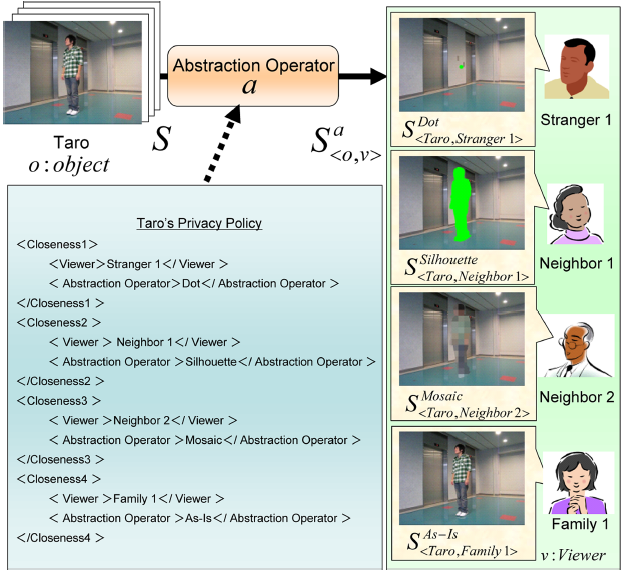
\includegraphics[width=.5\textwidth]{img//prisurv_simple_demo.png}}
\caption{PriSurv simple run case \cite{chinomi2008PriSurv}.}
\label{fig:prisurv}
\end{figure}

Figure~\ref{fig:prisurv} is an example run case of PriSurv, which shows how visual abstraction is used in order to protect the privacy of an object appearing within an image. Let o, a, v and S denote an object, an abstraction operator, a viewer and an original image, respectively. In the example, “Taro” is the object which appears within the original image and is monitored by “Stranger 1”, “Neighbor 1”, “Neighbor 2” and “Family 1” which are the different viewers. Since the closeness between the object and viewers is different, different abstraction operators are used for hiding the visual information of the object. In the example, these operators are “Dot”, “Silhouette”, “Mosaic” and “As-Is”, which are 4 of the 12 possible operators. Each viewer then receives a privacy protected version of the original image which is denoted by $S_{<o, v>}^a$. A simplified version of Taro’s privacy policy, which is a part of the abstraction operator, is also available to give a better understanding of how the closeness is defined. 

\subsubsection{System overview}

\begin{figure}[t]
\centerline{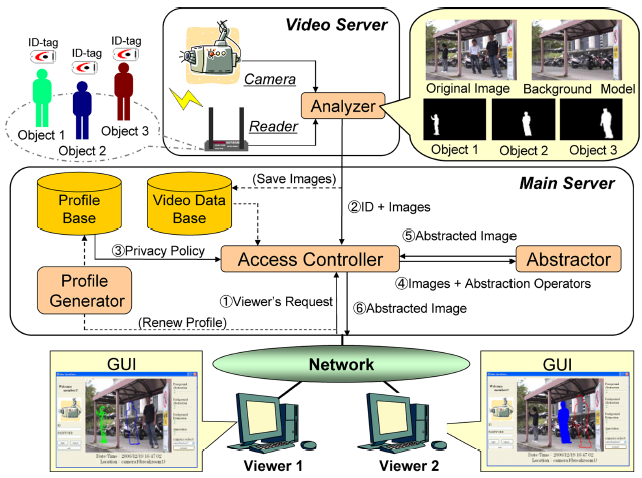
\includegraphics[width=.5\textwidth]{img//prisurv_arch.png}}
\caption{PriSurv system overview \cite{chinomi2008PriSurv}.}
\label{fig:prisurv2}
\end{figure}

Figure~\ref{fig:prisurv2} shows the architecture of the PriSurv system. It consists of three main parts: Video Server, Main Server and Network. It also has six different components: \textbf{Analyzer}, \textbf{Profile Generator}, \textbf{Profile Base}, \textbf{Access Controller}, \textbf{Abstractor} and \textbf{Video Data Base}. 

The \textbf{Analyzer}, which is a part of the video server, is responsible for identifying different objects. Each identifiable object must have its own \ac{RFID}-tag. The surveillance area is divided into smaller N x N areas and the location area of each \ac{RFID}-tag is determined by an \ac{RFID}-reader. Each object inside the original image is extracted and then identified separately by comparing the obtained visual data with the binary images of each object. 

The \textbf{Profile Generator} is used for setting up privacy policies for different members of the system. Each member's personal information such as name, age, gender and address and privacy policy is stored securely inside the \textbf{Profile Base}. The Profile Generator is also responsible for converting data taken from the GUI to \ac{XML}-based syntax. The profile of each member can only be updated by them and other members have no access to this data. 

The \textbf{Access Controller} determines the closeness relationship between a requesting viewer and an object to be monitored by reading the \ac{XML}-based privacy policies of the object stored inside the Profile Base. Once the types of abstraction operators are extracted, Access Controller sends them to the Abstractor. 

The \textbf{Abstractor} is a processor for images that performs visual abstraction by using abstraction operators. 

The \textbf{Video Data Base} stores past video data and makes it available to viewers after appropriate visual abstractions are performed. 

\subsection{Cardea Framework}

Surveillance cameras are not the only threat for the visual privacy of people. Availability of cameras within modern mobile and wearable devices has also increased people's concerns about their visual privacy, because nowadays taking photos or recording videos and then sharing online is easier. Moreover, sharing pictures and videos online could reveal more information than expected, especially when the data is publicly available. Usage of recognition technologies which are able to correlate the shared data to specific people, places, and things, could make the data searchable \cite{gross2014},\cite{shaw2006}. Even when taking photos is not involved, applications making use of the camera, such as \ac{AR} apps, could still compromise the visual privacy of bystanders by leaking the captured visuals, maliciously or not. 

Privacy issues raised by unnoticed or unauthorized collection of visuals have been addressed, both legally and technically. Google Glass, for instance, is not allowed to be used at places such as hospitals, bars, and movie theatres \cite{google2013glass}. However, banning such devices is not a good and fundamental solution, because it takes away the possibility of people to capture and share happy moments, especially if there are not any bystanders around. As a result, there are increasing needs to design technical solutions which can protect visual privacy of individuals while not restricting the rights of other individuals. 
	
There are proposals for using visual markers \cite{roesner2014},\cite{liu2014} or colourful hats \cite{sastry2007} with which people can declare their disagreement to be captured. These approaches, however, are not flexible enough, because people should be able to control, modify and express their individual privacy preferences naturally – without the need of any extra facilities. PriSurv system, which was discussed in the previous section, also relies on extra facilities such as \ac{RFID}-tags and -readers. Thus, it is not a feasible solution for built-in cameras. 

The Cardea framework \cite{shu2016cardea} does not rely on such or similar extra facilities, instead it takes advantage of computer vision techniques which are effective and reliable. Moreover, it allows people to change their privacy preferences dynamically, for example, by using predefined hand gestures. The framework also specifies context elements, such as scenes and presence of others. People can set their personal privacy profiles, hand gestures for flexible interaction with cameras and define context related privacy preferences. For example, some people might prefer their visual appearance to be hidden inside bars, but not in the parks. But in cases when they prefer to appear in photos, taken inside a bar, they can enable it with a hand gesture. Devices using the framework will automatically compute factors related to context, check people's privacy preferences, and protect their visual appearance by blurring their face.

\subsubsection{Key Concepts}
\begin{figure}[t]
\centerline{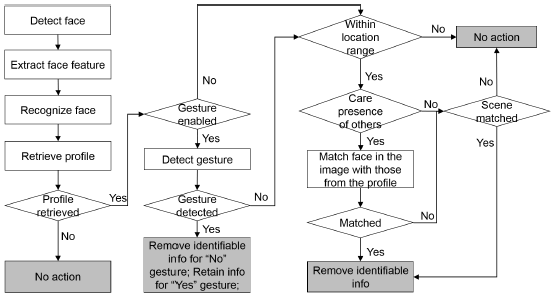
\includegraphics[width=.5\textwidth]{img/cardea_workflow.png}}
\caption{Cardea framework workflow \cite{shu2016cardea}.}
\label{fig:cardea}
\end{figure}

There are few key concepts which have to be briefly described before proceeding to the system overview. A person who has a device with integrated camera and is taking photos is the \textbf{recorder}. People who may appear in these photos are the \textbf{bystanders}. Bystanders who do not want to be identifiable in the photos can express their privacy preferences by using the Cardea framework. On the other hand, the recorder who cares and respects the privacy preferences of the bystanders can use the Cardea framework to take photos. Both the recorder and the bystanders are classified as \textbf{users} of the Cardea privacy protection framework. Each bystander sets their \textbf{privacy profile}. Each profile contains information such as \textbf{context elements}, \textbf{gesture interaction} options, and \textbf{privacy protection action} to be used. Bystanders have different privacy concerns depending on the context elements which can be locations, scenes and nearby people. The framework supports two gesture interactions: a victory sign and a palm, which stand for “Yes” and “No”, respectively, to the question “Would you like to appear in the taken photo?”. If a bystander does not use any of these gestures while the photo is taken, then the default privacy settings set in the privacy profile apply. Action taken in order to protect the visual privacy is face blurring. But further methods such as full body blurring, blending the body region into the background, or replacing the face with an average face are possible to be integrated. All preferences of the bystanders are stored inside a \textbf{cloud} which accepts requests from the recorder and processes images in a such way that the privacy preferences of the bystanders appearing in the images is respected. Figure~\ref{fig:cardea} visualizes the decision workflow of the Cardea framework. Decisions are made according to the computing results from the camera and remote cloud, then the original image is processed, in case it contradicts the privacy preferences of the bystanders. 

\subsubsection{System Overview}
\begin{figure}[t]
\centerline{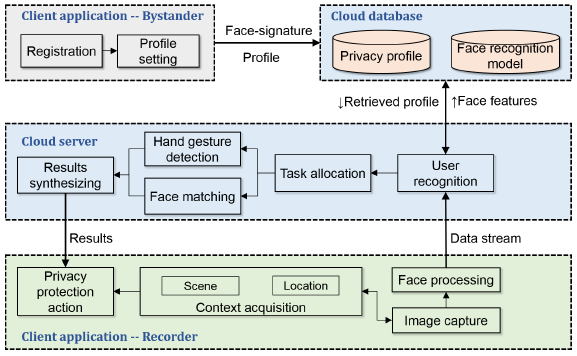
\includegraphics[width=.5\textwidth]{img/cardea_overview_diagram.png}}
\caption{Cardea framework system overview \cite{shu2016cardea}.}
\label{fig:cardea2}
\end{figure}

Figure~\ref{fig:cardea2} shows the interactions between the major components. Cardea is composed of the client app and the cloud server. Bystanders can register, setup their profile settings and upload their photo by using the user interface of the client application. Face features of the bystander will be extracted and stored into the cloud server's database and be used for training the face recognition model. The privacy profile will also be stored in the database. Bystanders can change their privacy preferences at any time later. 

Recorders use the client application to take photos. The application detects faces in the taken photos, extracts face features and computes context elements on the device. Face matching, user recognition and hand gesture detection processes are done on the cloud server, because they are computationally-intensive and infeasible on most devices. Once the results from the cloud are received, protection action will be performed. 

The cloud server is responsible for storing user profiles and processing detection tasks upon requests from the recorder side. User recognition process is divided into three steps. The first step is to detect face regions on the image and then filter the results in order to reduce false positives. The second step is to extract face features in a compact but still discriminative way, so the face detection is done using these features rather than comparing just raw pixels. The last step is to match these representative features to faces stored on the cloud database. 

Location filtering feature helps users define specific locations in which they may worry about their privacy more. The location of the device taking a picture is obtained directly from the \ac{GPS}. Scene classification is a more complex concept, because it does not only rely to places, but also gives information about the current activities of people. The framework covers 9 general scene groups which are further divided into more specific scenes. In total there are 98 different scenes. Users can more easily specify their privacy preferences by selecting from these general scene groups. 


\subsubsection{Example run case and evaluations}
\begin{figure}[t]
\centerline{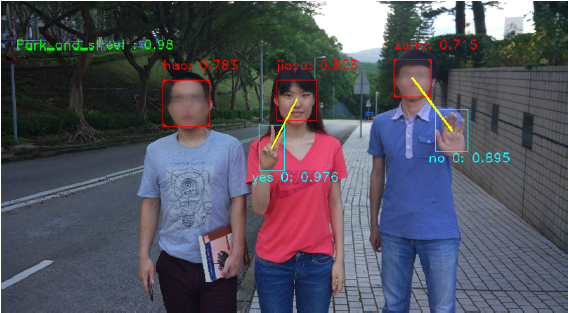
\includegraphics[width=.5\textwidth]{img/cardea_example.png}}
\caption{Cardea framework example run case \cite{shu2016cardea}.}
\label{fig:cardea3}
\end{figure}

Figure~\ref{fig:cardea3} shows a privacy protection example of the Cardea framework. The framework is able to detect three registered users, two hand gestures and a scene. The scene is classified correctly as Park \& street. The face of Hao is detected and blurred by default in order to match his visual privacy preferences. The face of Zerry, under normal circumstances, would not have been blurred, but because he is using “No” gesture while this particular picture is taken, his face is blurred. Jiayu has the opposite case of Zerry. Under normal circumstances her face would have been blurred, but because of her “Yes” gesture her face is identifiable.



\subsection{Sharing of Multi-Subject and Interdependent Data}
Reference \cite{olteanu2018consensual}


\subsection{Others - More specific Audio or Location based technologies should be found}


\section{Limitations and challenges of privacy ensuring technologies}\label{Limitations}
\subsection{Cardea (user contribution)}
Willingly putting your personal data on a cloud to avoid having your privacy invaded by others can be seen as counter productive
\subsection{Example 2}
\subsection{Example 3}
\subsection{(optionally) Ideas that could fix these limitations}

\section{Conclusion}\label{Conclusion}


\begin{table}[htbp]
\caption{Table Type Styles}
\begin{center}
\begin{tabular}{|c|c|c|c|}
\hline
\textbf{Table}&\multicolumn{3}{|c|}{\textbf{Table Column Head}} \\
\cline{2-4} 
\textbf{Head} & \textbf{\textit{Table column subhead}}& \textbf{\textit{Subhead}}& \textbf{\textit{Subhead}} \\
\hline
copy& More table copy$^{\mathrm{a}}$& &  \\
\hline
\multicolumn{4}{l}{$^{\mathrm{a}}$Sample of a Table footnote.}
\end{tabular}
\label{tab1}
\end{center}
\end{table}

\section*{Abbreviations and Acronyms}
\addcontentsline{toc}{section}{Abbreviations and Acronyms}
\begin{acronym}[Bash]
\acro{IoT} {\textit{Internet of Things}}
\acro{AR} {\textit{Augmented Reality}}
\acro{RFID} {\textit{Radio-frequency identification}}
\acro{XML} {\textit{Extensible Markup Language}}
\acro{GPS} {\textit{Global Positioning System}}
\end{acronym}

\bibliographystyle{IEEEtran}
{\footnotesize
\bibliography{literature_list}}

\end{document}